\documentclass{beamer}

\usepackage[utf8]{inputenc}
\usetheme{Madrid}
\usecolortheme{beaver}

\usepackage{graphicx}
\graphicspath{ {./Resources/} }

% Title here
\title{Sample Presentation}
\author{Unamed Team}
\institute{SNHU/CETA, EG-310}


\usepackage[utf8]{inputenc}
\usetheme{Madrid}
\usecolortheme{beaver}

\usepackage{graphicx}
\graphicspath{ {./Resources/} }

% Title here
\title{Sample Presentation}
\author{Tim, Ben, Joe, Max}
\institute{SNHU/CETA, EG-310}

\begin{document}

\frame{\titlepage} % Draw the title page

% A frame
\begin{frame}
    \frametitle{Network}

    % Some columns
    \begin{columns}
        \begin{column}{0.48\textwidth}
            \begin{block}{Cute critter}
                What is this thing?
            \end{block}
        \end{column}
        \begin{column}{0.48\textwidth}
            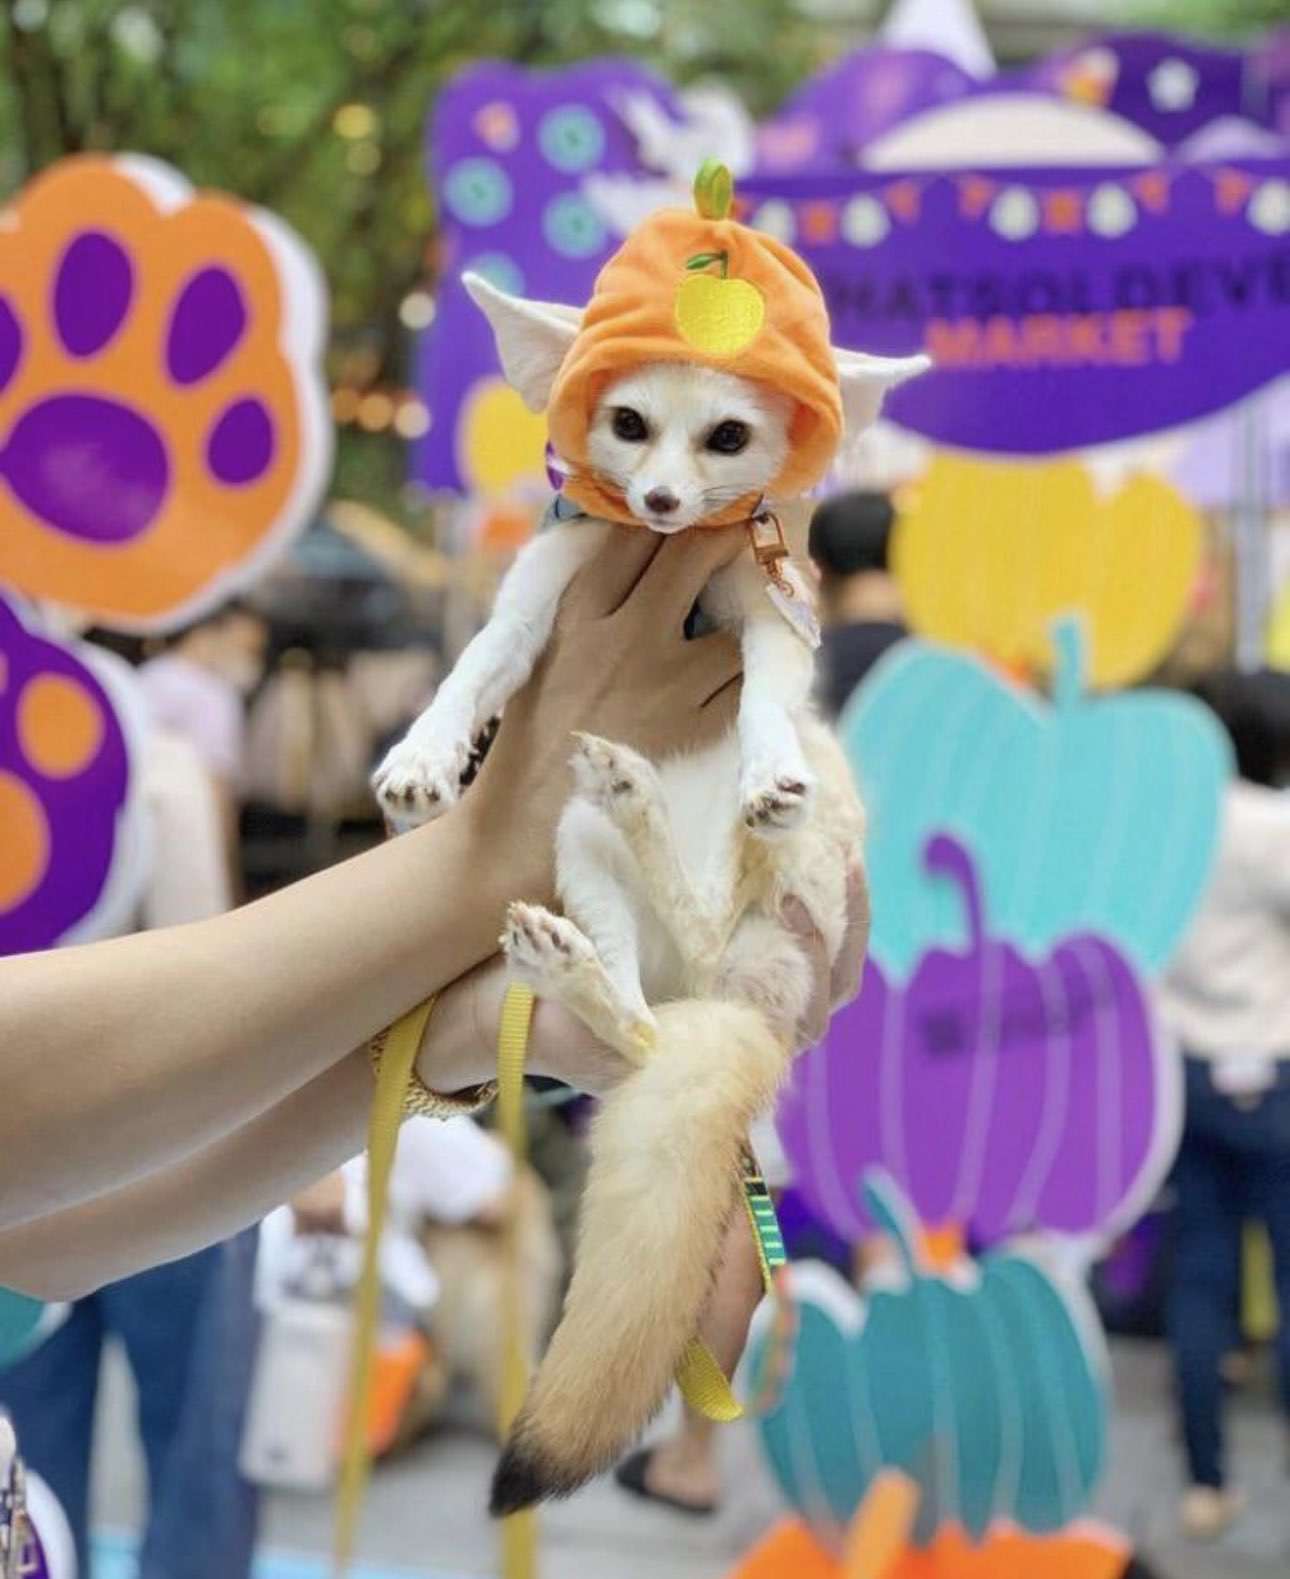
\includegraphics[width=5cm]{what_is_this_thing}
        \end{column}
    \end{columns}

\end{frame}


% A frame
\begin{frame}
    \frametitle{Features}



    \begin{block}{\centering C\# Was Used to Develop the Following Features:}
        \centering User Connection, Class Selection, Note Selection, Add Note
    \end{block}

    \centering 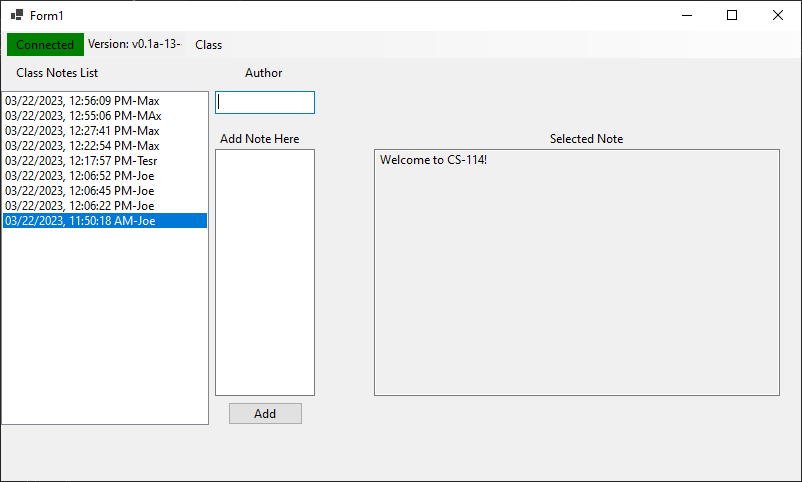
\includegraphics[height=6cm]{Sample_of_Features.PNG}

\end{frame}

\begin{frame}
    \frametitle{User Interface}

    % Some columns
    \begin{columns}
        \begin{column}{0.48\textwidth}
            \begin{block}{Cute critter}
                What is this thing?
            \end{block}
        \end{column}
        \begin{column}{0.48\textwidth}
            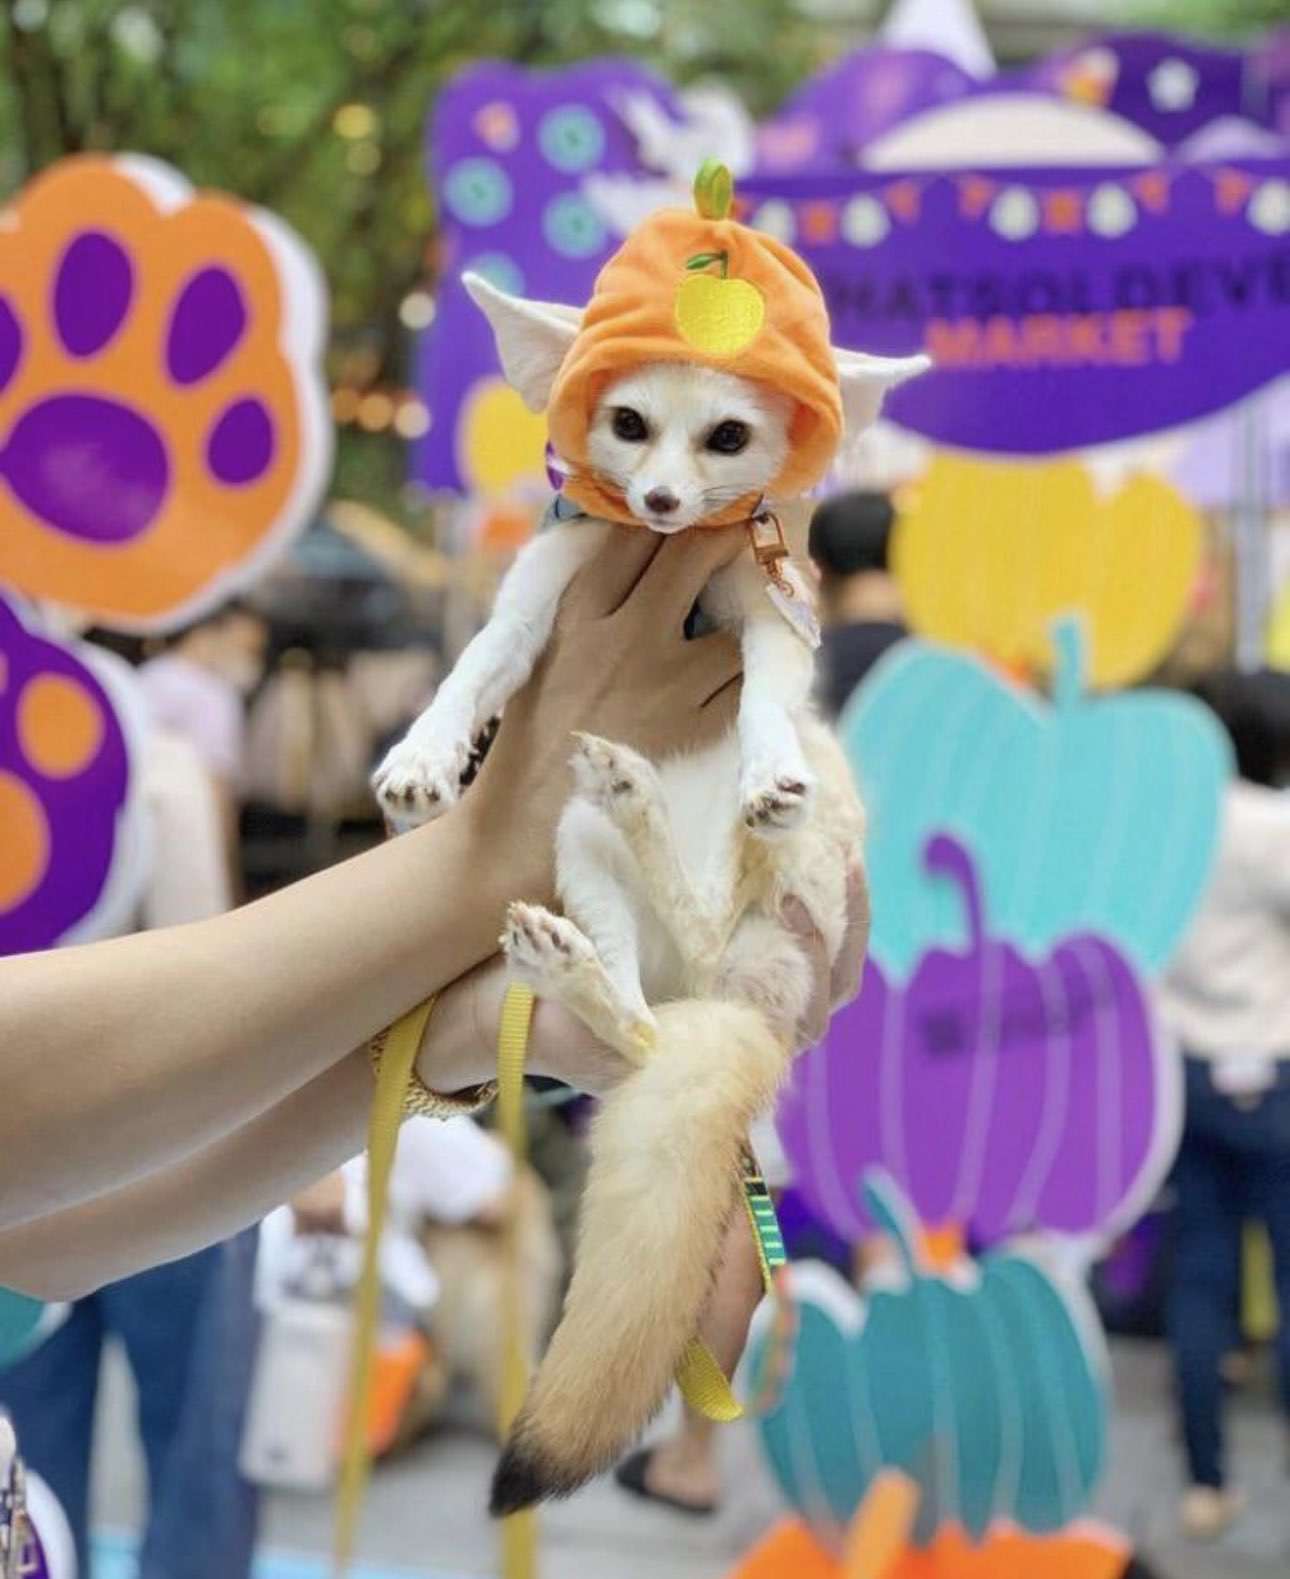
\includegraphics[width=5cm]{what_is_this_thing}
        \end{column}
    \end{columns}

\end{frame}

\end{document}

